\documentclass[a4paper,10pt]{article}

\usepackage[brazilian]{babel}
\usepackage[utf8]{inputenc}
\usepackage[T1]{fontenc}
\usepackage{titlesec}
\usepackage{graphicx}
\usepackage{mathtools}
\usepackage{amsthm}
\usepackage[top=1.0in,bottom=1.0in]{geometry}
\usepackage{hyperref}
\usepackage[singlelinecheck=false]{caption}
\usepackage[backend=biber,url=true,doi=true,eprint=false]{biblatex}

\addbibresource{references.bib}

\newcommand\blfootnote[1]{%
  \begingroup
  \renewcommand\thefootnote{}\footnote{#1}%
  \addtocounter{footnote}{-1}%
  \endgroup
}

\titleformat{\section}
  {\normalfont\scshape\bfseries}{\thesection}{1em}{}
\titleformat{\subsection}
  {\normalfont\scshape\bfseries}{\thesubsection}{1em}{}
\titleformat{\paragraph}
  {\normalfont}{\theparagraph}{1em}{}
\titleformat{\subparagraph}
  {\normalfont}{\thesubparagraph}{1em}{}

\captionsetup[table]{labelsep=space}

\theoremstyle{plain}

\newtheorem*{spn-def}{Definição}

\title{\textbf{Aprendizado Automático de Sum-Product Networks (SPN)}}

\begin{document}
\date{}
\author{}
\vspace*{-40pt}
{\let\newpage\relax\maketitle}

Projeto de MAC0215 (Atividade Curricular em Pesquisa)

Aluno: Renato Lui Geh (Bacharelado em Ciência da Computação)

Orientador: Denis Deratani Mauá

\section{Introdução}

\paragraph{
  Para compreendermos melhor as aplicações de uma Sum-Product Network precisamos primeiro entendermos distribuições
de probabilidade multivariadas, o que é o escopo de uma distribuição, as dificuldades de representar todas as 
probabilidades no espaço e o que é inferência de uma distribuição.
}

\subsection{Distribuições de probabilidade multivariadas}

\paragraph{
  Uma distribuição de probabilidade multivariada é uma distribuição de probabilidade que resulta na probabilidade 
de que cada variável aleatória $X_1,...,X_n$, para $n\geq{2}$, esteja em um dado intervalo ou conjunto para cada valor 
$x_i$, $1\leq{i}\geq{n}$ correspondente. Se a distribuição possui apenas uma variável aleatória, dizemos que ela é uma
distribuição de probabilidade monovariável. Um exemplo de distribuição multivariada segue abaixo:
}

\paragraph{
  Consideremos um dado não viciado. Seja $A=1$ se o número tirado é par e $A=0$ caso contrário. Seja $B=1$ se o
mesmo número tirado em $A$ é primo e $B=0$ caso contrário. Podemos construir a tabela abaixo:
}

\begin{table}[h]
\caption{}
\begin{tabular}{l | *{6}{c}}
  & 1 & 2 & 3 & 4 & 5 & 6 \\
\hline
A & 0 & 1 & 0 & 1 & 0 & 1 \\
B & 0 & 1 & 1 & 0 & 1 & 0 \\
\end{tabular}
\end{table}

\paragraph{
  A distribuição de probabilidade multivariada resultante é:
}

\subparagraph{$P(A=0,B=0) = P\{1\} = \frac{1}{6}$ \\
  $P(A=1,B=0) = P\{4,6\} = \frac{2}{6}$ \\
  $P(A=0,B=1) = P\{3,5\} = \frac{2}{6}$ \\
  $P(A=1,B=1) = P\{2\} = \frac{1}{6}$
} 

\subsection{Escopo de uma distribuição}

\paragraph{
  Denotamos $P(X_1=x_1,...,X_n=x_n)$, dados valores $x_1,...,x_n$, uma distribuição de probabilidade multivariada
com variáveis aleatórias $X_1,...,X_n$. Dada uma distribuição de probabilidade, chamamos de escopo da distribuição 
o conjunto de variáveis que definem o domínio da função, ou seja, $X_1,...,X_n$. No caso da Tabela 1, o escopo da 
probabilidade é o conjunto $\{A, B\}$. 
}

\begin{spn-def} Sejam $P_1 (X_1,...,X_k)$ e $P_2 (X_k,...,Y_n)$ distribuições de probabilidade multivariadas cujos
  escopos têm mesmo tamanho.
\begin{enumerate} \itemsep0pt
  \item Dizemos que $P_1$ e $P_2$ tem mesmo escopo se para toda variável aleatória $X_i$ em $P_1$ existe uma
variável aleatória $X_j$ em $P_2$ tal que $i=j$.
  \item Dizemos que $P_1$ e $P_2$ tem escopos disjuntos se para qualquer variável aleatória $X_i$ em $P_1$,
toda variável aleatória $X_j$ em $P_2$ obedece a regra $i\neq{j}$. 
\end{enumerate}
\end{spn-def}

\subsection{Espaço de uma distribuição multivariada}

\paragraph{
  Vamos reutilizar a Tabela 1, renomeando $A$ para $X_1$ e $B$ para $X_2$. Portanto teremos $P(X_1=x_1,X_2=x_2)$. 
Montando a tabela temos que:
}

\begin{table}[h*]
\caption{}
\begin{tabular}{*{3}{c}}
$X_1$ & $X_2$ & $P(X_1=x_1,X_2=x_2)$ \\
\hline
$X_1=0$ & $X_2=0$ & $\frac{1}{6}$ \\
$X_1=0$ & $X_2=1$ & $\frac{2}{6}$ \\
$X_1=1$ & $X_2=0$ & $\frac{2}{6}$ \\
$X_1=1$ & $X_2=1$ & $\frac{1}{6}$ \\
\end{tabular}
\end{table}

\paragraph{
  Pode-se ver que uma tabela com todas as possíveis probabilidades de todas as variáveis terá $2^n$ elementos, 
onde $n$ é o número de variáveis aleatórias. Portanto o crescimento em espaço necessário é exponencial, o que
é impraticável em conjuntos de dados maiores. A solução vem com o uso de Redes Profundas (ex.: Sum-Product Networks), 
que tornam $O(2^n)$ em $O(n)$ no tamanho do grafo.
}

\subsection{Inferência}



\section{Definição}

\paragraph{
  Sum-Product Networks são uma nova classe de modelos probabilísticos cuja inferência é sempre
polinomial no tamanho da rede.
}

\begin{spn-def} Uma SPN é recursivamente, pela definição de Gens e Domingos\cite{gens-domingos}:
\begin{enumerate} \itemsep0pt
  \item Uma distribuição monovariável polinomial.
  \item Um produto de SPNs cujos escopos são disjuntos.
  \item Uma soma de SPNs com peso não negativo cujos elementos tem mesmo escopo.
  \item Nada mais é uma SPN.
\end{enumerate}
\end{spn-def}

\paragraph{
  Podemos definir graficamente uma SPN como um grafo direcionado acíclico (DAG) onde as 
folhas são sempre variáveis (ou distribuições monovariáveis), seus nós internos são somas ou 
produtos e para todo vértice conectando um nó soma com um nó filho há um peso não negativo. 
Também assume-se que toda soma e produto estão em alturas alternantes, ou seja, todo nó pai 
de um nó interno que é soma é um produto e vice-versa.
}

\begin{figure}[h]
\centering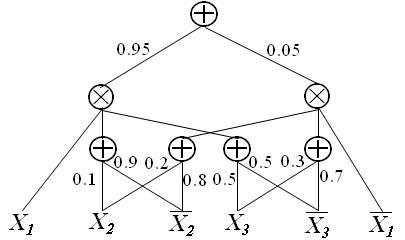
\includegraphics[scale=0.7]{imgs/domingos_poon.jpg}
\caption{Um exemplo de uma SPN com variáveis Booleanas, onde $x_1,...,x_d$ e 
  $\overline{x_1},...,\overline{x_d}$ são folhas e o resto dos nós são somas ou produtos.\cite{poon-domingos}}
\end{figure}

Dada uma distribuição multivariada, podemos construir uma SPN. 

\section{Características}

\paragraph{
  Há várias vantagens de SPNs sobre outras redes de aprendizado:
}

\begin{enumerate} \itemsep0pt
  \item SPNs tem estrutura parecida a outros Modelos Gráficos Probabilisticos (PGM), mas a 
    representação de certos tipos de independência é mais fácil.
  \item SPNs tem inferência polinomial no tamanho do grafo, enquanto que inferência em Redes Bayesianas
    é NP-difícil.
  \item Experimentos mostram que aprendizado de arquiteturas SPN tiveram melhores resultados quando
    comparadas a arquiteturas estáticas.\cite{clustering}
\end{enumerate}

\section{Aplicações}

SPNs obtiveram resultados impressionantes em muitos conjuntos de dados\cite{website:spn-uwashington}, tais como:

\begin{itemize} \itemsep0pt
  \item Reconstrução de imagens.
  \item Classificação.
  \item Reconhecimento de atividade.
  \item Logs click-through.
  \item Sequências de ácido nucleico.
  \item Filtragem colaborativa.
\end{itemize}

\section{Proposta}

\paragraph{
  O objetivo deste projeto é realizar uma comparação das principais técnicas de aprendizado 
automático de Sum-Product Network a partir de um conjunto de dados, avaliando o desempenho 
e os resultados das técnicas utilizadas.
}

\paragraph{
  Será estudada a estrutura e propriedades de uma Sum-Product Network e em seguida
aplicada as seguintes técnicas de aprendizado:
}

\begin{itemize} \itemsep0pt
  \item Divisão em subconjuntos mutualmente independentes e EM clustering.\cite{gens-domingos}  
  \item Busca gulosa.\cite{greedy-search}
  \item Aprendizado com clustering de variáveis.\cite{clustering}
  \item Aprendizado por meio de SPNs Bayesianas Não-Paramétricas.\cite{non-parametric-bayesian}
\end{itemize}

\paragraph{
  Em seguida o aluno irá comparar as técnicas implementadas e apresentar os resultados.
}

\section{Acompanhamento}

\paragraph{
  Relatórios semanais serão publicados no seguinte endereço: 
}

\subparagraph{\url{http://www.ime.usp.br/~renatolg/mac0215/doc/reports/}}

\paragraph{
  É também possível acompanhar tanto os relatórios quanto as implementações pelo repositório
do projeto:
}

\subparagraph{\url{https://github.com/RenatoGeh/mac0215/}}

\newpage

\section{Referências}

\printbibliography[title={Artigos},type=article]
\printbibliography[title={Websites},type=misc]

\blfootnote{Os artigos listados na referência acima podem ser encontrados em: 
  \url{http://www.ime.usp.br/~renatolg/mac0215/articles/}}

\end{document}
